\documentclass[twoside]{book}

% Packages required by doxygen
\usepackage{fixltx2e}
\usepackage{calc}
\usepackage{doxygen}
\usepackage[export]{adjustbox} % also loads graphicx
\usepackage{graphicx}
\usepackage[utf8]{inputenc}
\usepackage{makeidx}
\usepackage{multicol}
\usepackage{multirow}
\PassOptionsToPackage{warn}{textcomp}
\usepackage{textcomp}
\usepackage[nointegrals]{wasysym}
\usepackage[table]{xcolor}

% Font selection
\usepackage[T1]{fontenc}
\usepackage[scaled=.90]{helvet}
\usepackage{courier}
\usepackage{amssymb}
\usepackage{sectsty}
\renewcommand{\familydefault}{\sfdefault}
\allsectionsfont{%
  \fontseries{bc}\selectfont%
  \color{darkgray}%
}
\renewcommand{\DoxyLabelFont}{%
  \fontseries{bc}\selectfont%
  \color{darkgray}%
}
\newcommand{\+}{\discretionary{\mbox{\scriptsize$\hookleftarrow$}}{}{}}

% Page & text layout
\usepackage{geometry}
\geometry{%
  a4paper,%
  top=2.5cm,%
  bottom=2.5cm,%
  left=2.5cm,%
  right=2.5cm%
}
\tolerance=750
\hfuzz=15pt
\hbadness=750
\setlength{\emergencystretch}{15pt}
\setlength{\parindent}{0cm}
\setlength{\parskip}{3ex plus 2ex minus 2ex}
\makeatletter
\renewcommand{\paragraph}{%
  \@startsection{paragraph}{4}{0ex}{-1.0ex}{1.0ex}{%
    \normalfont\normalsize\bfseries\SS@parafont%
  }%
}
\renewcommand{\subparagraph}{%
  \@startsection{subparagraph}{5}{0ex}{-1.0ex}{1.0ex}{%
    \normalfont\normalsize\bfseries\SS@subparafont%
  }%
}
\makeatother

% Headers & footers
\usepackage{fancyhdr}
\pagestyle{fancyplain}
\fancyhead[LE]{\fancyplain{}{\bfseries\thepage}}
\fancyhead[CE]{\fancyplain{}{}}
\fancyhead[RE]{\fancyplain{}{\bfseries\leftmark}}
\fancyhead[LO]{\fancyplain{}{\bfseries\rightmark}}
\fancyhead[CO]{\fancyplain{}{}}
\fancyhead[RO]{\fancyplain{}{\bfseries\thepage}}
\fancyfoot[LE]{\fancyplain{}{}}
\fancyfoot[CE]{\fancyplain{}{}}
\fancyfoot[RE]{\fancyplain{}{\bfseries\scriptsize Generated by Doxygen }}
\fancyfoot[LO]{\fancyplain{}{\bfseries\scriptsize Generated by Doxygen }}
\fancyfoot[CO]{\fancyplain{}{}}
\fancyfoot[RO]{\fancyplain{}{}}
\renewcommand{\footrulewidth}{0.4pt}
\renewcommand{\chaptermark}[1]{%
  \markboth{#1}{}%
}
\renewcommand{\sectionmark}[1]{%
  \markright{\thesection\ #1}%
}

% Indices & bibliography
\usepackage{natbib}
\usepackage[titles]{tocloft}
\setcounter{tocdepth}{3}
\setcounter{secnumdepth}{5}
\makeindex

% Custom commands
\newcommand{\clearemptydoublepage}{%
  \newpage{\pagestyle{empty}\cleardoublepage}%
}

\usepackage{caption}
\captionsetup{labelsep=space,justification=centering,font={bf},singlelinecheck=off,skip=4pt,position=top}

%===== C O N T E N T S =====

\begin{document}

% Titlepage & ToC
\pagenumbering{alph}
\begin{titlepage}
\vspace*{7cm}
\begin{center}%
{\Large Projeto 03 \\[1ex]\large 01 }\\
\vspace*{1cm}
{\large Generated by Doxygen 1.8.14}\\
\end{center}
\end{titlepage}
\clearemptydoublepage
\pagenumbering{roman}
\tableofcontents
\clearemptydoublepage
\pagenumbering{arabic}

%--- Begin generated contents ---
\chapter{Projeto de Programação}
\label{md__c_1__users__dorgival__desktop__projeto03__r_e_a_d_m_e}
\subsection*{Apresentação}

O presente projeto visa desenvolver o aluno na prática de programação orientada a objetos usando a biblioteca Qt.

O projeto consiste em três programas de computador que trabalham em conjunto para simular um sistema simples de aquisição e supervisão de dados usando comunicação T\+C\+P/\+IP em uma rede local.

Em suma, os três módulos devem ser capazes de realizar as seguintes operações\+:


\begin{DoxyItemize}
\item O {\bfseries servidor} deve esperar conexões T\+CP destinadas à porta 1234, e responder ao cliente conforme os comandos que este enviar.
\item O {\bfseries cliente produtor} de dados deve ser capaz de se conectar a uma máquina executando o servidor na porta 1234 e enviar, usando comandos específicos, marcações de data/hora juntamente com uma informação em ponto flutuante para ser gravada.
\item O {\bfseries cliente supervisor} de dados deve ser capaz de se conectar a uma máquina executando o servidor na porta 1234 e recuperar, usando comandos específicos, a lista dos clientes produtores de dados, bem como listagens de dados produzidos por um destes clientes produtores.
\end{DoxyItemize}

O aluno deverá desenvolver apenas os {\bfseries cliente produtor} e o {\bfseries cliente supervisor}. O módulo {\bfseries servidor} já está pronto e não precisa ser trabalhado.

\subsection*{O módulo servidor}

O módulo servidor implementa o que se chama de servidor T\+CP. Em outras palavras, esse programa é capaz de escutar a rede local e aguardar por conexões remotas destinadas à porta T\+C\+P/1234.

Em redes T\+C\+P/\+IP, o protocolo de comunicação T\+CP permite a criação de um circuito virtual, um canal de comunicação que pode ser usado para enviar e receber sequências de bytes pela Internet. O canal é fechado apenas quando a conexão é interrompida.

Para se abrir uma conexão com uma máquina que executa um determinado serviço usando o protocolo T\+CP é necessário que se conheça seu endereço IP (ou nome) e uma {\itshape porta} onde o serviço será provido. Quando a conexão é aberta para um novo cliente, inicia-\/se um {\itshape socket} de comunicação, identificado, entre outras coisas, pela combinação I\+P+porta. Cada {\itshape socket} possui um número único que pode ser usado para distinguir entre as várias conexões que podem chegar à mesma porta. Isso é comum em máquinas que provêem serviços a vários clientes.

Máquinas que aguardam conexões comumente chamadas de {\bfseries servidores}. O servidor implementado neste projeto {\itshape escuta} a porta {\bfseries 1234}. Uma vez que um cliente se conecte a esta, as tarefas que o servidor irá executar dependerão de mensagens enviadas pelo cliente. Para cada mensagem, uma tarefa diferente é executada. É dessa maneira que os vários serviços na Internet funcionam.

O servidor do projeto não necessita de modificações para funcionar. Basta abrir o projeto no Qt\+Creator, compilar e executar o código. O servidor é capaz de interpretar mensagens em texto simples que lhe forem enviadas. As mensagens aceitas pelo servidor formam o que se chama de {\bfseries protocolo de aplicação} para este serviço. Três mensagens são suportadas nesse protocolo\+:


\begin{DoxyCode}
list
get NUMERO\_IP N\_AMOSTRAS
set DATA\_E\_HORA\_EM\_MS DADO
\end{DoxyCode}


O comando $\ast$$\ast$\+\_\+list\+\_\+$\ast$$\ast$ retorna a lista de máquinas cujos dados produzidos encontram-\/se armazenados no servidor. ex\+: 
\begin{DoxyCode}
$ telnet 127.0.0.1 1234
list
127.0.0.1
\end{DoxyCode}


O comando $\ast$$\ast$\+\_\+get\+\_\+$\ast$$\ast$ precisa que se forneça também o número IP do {\bfseries cliente produtor} que se deseja recuperar o conjunto de dados produzidos. ex\+:


\begin{DoxyCode}
$ telnet 127.0.0.1 1234
get 127.0.0.1 1
1496658174409 34
\end{DoxyCode}


O comando $\ast$$\ast$\+\_\+set\+\_\+$\ast$$\ast$ precisa que se forneça uma combinação D\+A\+TA e H\+O\+RA, bem como o dado que se deseja armazenar no servidor. ex\+:


\begin{DoxyCode}
$ telnet 127.0.0.1 1234
set 127.0.0.1
set 1496658174409 34
\end{DoxyCode}


Todos os comandos devem ser enviados na forma de literais. O indicador de data/hora é um long que armazena a quantidade de milisegundos passados desde a data 1/1/1970. O servidor, uma vez que receba essas sequências de literais, separa-\/as conforme a quantidade de espaços presentes e armazena os dados associados em uma estrutura local criada para esse fim.

Em se tratando de um projeto meramente acadêmico, pouco controle de erro é realizado nessa versão inicial.

Quando o servidor é executado, uma mensagem é exibida na aba {\bfseries Application Output} do Qt\+Creator mostrando o IP local do servidor, como ilustram as linhas a seguir\+:


\begin{DoxyCode}
server started at:
"192.168.1.106"
\end{DoxyCode}


\subsection*{O módulo cliente produtor de dados}

O cliente produtor de dados deve ser capaz de se conectar a um servidor em execução e enviar comandos {\bfseries set} para este servidor. Espera-\/se que esse módulo seja capaz de simular um processo de coleta e envio de dados para o servidor em intervalos periódicos.

A construção do cliente deve possibilitar o envio de dados (possivelmente aleatórios) para o servidor em intervalos regulares de tempo. Para isso, seu usuário deverá ser capaz de realizar as seguintes operações no módulo produtor\+:


\begin{DoxyItemize}
\item Indicar o IP do servidor ao qual se deseja conectar
\item Indicar a faixa de valores (min-\/max) que poderão ser enviados ao servidor
\item Indicar o intervalo de tempo entre o envio de dois dados consecutivos
\item Realizar a conexão ao pressionar um botão
\item Iniciar a transmissão de dados ao pressionar um botão
\item Finalizar a transmissão de dados ao pressionar um botão
\item Exibir os dados enviados em uma janela de texto
\end{DoxyItemize}

Um exemplo de interface para o módulo produtor de dados é mostrado na figura que segue\+:



\subsection*{Consumidor de dados}

O consumidor de dados assume um papel mais complexo que o produtor. O produtor deve ser capaz de se conectar a um servidor indicado, recuperar os endereços das máquinas que produziram dados e traçar um gráfico data-\/hora x valor de uma sequência de dados fornecida pelo servidor.

O usuário do módulo consumidor de dados, o usuário deverá ter à sua disposição as seguintes funcionalidades\+:


\begin{DoxyItemize}
\item Indicar o endereço IP do servidor de dados ao qual o cliente deverá se conectar.
\item Iniciar a conexão com o servidor ao se pressionar um botão.
\item Uma vez conectado, o usuário deverá ter a disposição uma lista das máquinas que produziram dados no servidor. Isso pode ser implementado usando um {\bfseries listwidget}.
\item No {\bfseries listwidget} o usuário deverá ser capaz de selecionar a máquina cujos dados deseja visualizar.
\item Com uma máquina selecionada, dois botões deverão ficar disponíveis para o usuário\+: um para começar a receber os dados e outro para parar de receber.
\item Deverá ficar disponível a possibilidade de modificar o intervalo de tempo de captura entre dois conjuntos de dados consecutivos, ou seja, entre o envio de dois comandos \+\_\+get 
\end{DoxyItemize}

Para cada recepção de dados, a ferramenta deverá traçar o gráfico tempo x valor do conjunto de dados lido do servidor. Algumas formas de traçado podem ser consideradas\+:


\begin{DoxyItemize}
\item Traçar todo intervalo de valores lido do servidor.
\item Traçar um subintervalo dos valores lidos (ex\+: desenhar apenas as últimas 30 amostras obtidas). Isso pode interessante para evitar que o gráfico fique sobrecarregado.
\end{DoxyItemize}

Um exemplo de interface para o módulo consumidor de dados é mostrado na figura que segue\+:

 
\chapter{Namespace Index}
\section{Namespace List}
Here is a list of all documented namespaces with brief descriptions\+:\begin{DoxyCompactList}
\item\contentsline{section}{\mbox{\hyperlink{namespace_ui}{Ui}} \\*The \mbox{\hyperlink{class_ui_1_1_main_window}{Main\+Window}} class tem a função de desenhar a interface }{\pageref{namespace_ui}}{}
\end{DoxyCompactList}

\chapter{Hierarchical Index}
\section{Class Hierarchy}
This inheritance list is sorted roughly, but not completely, alphabetically\+:\begin{DoxyCompactList}
\item \contentsline{section}{Data\+Storage}{\pageref{class_data_storage}}{}
\item \contentsline{section}{Entry}{\pageref{struct_entry}}{}
\item Q\+Main\+Window\begin{DoxyCompactList}
\item \contentsline{section}{Main\+Window}{\pageref{class_main_window}}{}
\item \contentsline{section}{Main\+Window}{\pageref{class_main_window}}{}
\item \contentsline{section}{Main\+Window}{\pageref{class_main_window}}{}
\item \contentsline{section}{Main\+Window}{\pageref{class_main_window}}{}
\end{DoxyCompactList}
\item \contentsline{section}{qt\+\_\+meta\+\_\+stringdata\+\_\+\+Main\+Window\+\_\+t}{\pageref{structqt__meta__stringdata___main_window__t}}{}
\item \contentsline{section}{qt\+\_\+meta\+\_\+stringdata\+\_\+\+My\+Server\+\_\+t}{\pageref{structqt__meta__stringdata___my_server__t}}{}
\item \contentsline{section}{qt\+\_\+meta\+\_\+stringdata\+\_\+\+My\+Thread\+\_\+t}{\pageref{structqt__meta__stringdata___my_thread__t}}{}
\item Q\+Tcp\+Server\begin{DoxyCompactList}
\item \contentsline{section}{My\+Server}{\pageref{class_my_server}}{}
\end{DoxyCompactList}
\item Q\+Thread\begin{DoxyCompactList}
\item \contentsline{section}{My\+Thread}{\pageref{class_my_thread}}{}
\end{DoxyCompactList}
\item \contentsline{section}{Range\+Test}{\pageref{struct_range_test}}{}
\item \contentsline{section}{Ui\+\_\+\+Main\+Window}{\pageref{class_ui___main_window}}{}
\begin{DoxyCompactList}
\item \contentsline{section}{Ui\+:\+:Main\+Window}{\pageref{class_ui_1_1_main_window}}{}
\item \contentsline{section}{Ui\+:\+:Main\+Window}{\pageref{class_ui_1_1_main_window}}{}
\item \contentsline{section}{Ui\+:\+:Main\+Window}{\pageref{class_ui_1_1_main_window}}{}
\item \contentsline{section}{Ui\+:\+:Main\+Window}{\pageref{class_ui_1_1_main_window}}{}
\item \contentsline{section}{Ui\+:\+:Main\+Window}{\pageref{class_ui_1_1_main_window}}{}
\item \contentsline{section}{Ui\+:\+:Main\+Window}{\pageref{class_ui_1_1_main_window}}{}
\item \contentsline{section}{Ui\+:\+:Main\+Window}{\pageref{class_ui_1_1_main_window}}{}
\end{DoxyCompactList}
\end{DoxyCompactList}

\chapter{Class Index}
\section{Class List}
Here are the classes, structs, unions and interfaces with brief descriptions\+:\begin{DoxyCompactList}
\item\contentsline{section}{\mbox{\hyperlink{class_data_storage}{Data\+Storage}} }{\pageref{class_data_storage}}{}
\item\contentsline{section}{\mbox{\hyperlink{struct_entry}{Entry}} }{\pageref{struct_entry}}{}
\item\contentsline{section}{\mbox{\hyperlink{class_main_window}{Main\+Window}} \\*The \mbox{\hyperlink{class_main_window}{Main\+Window}} class }{\pageref{class_main_window}}{}
\item\contentsline{section}{\mbox{\hyperlink{class_ui_1_1_main_window}{Ui\+::\+Main\+Window}} }{\pageref{class_ui_1_1_main_window}}{}
\item\contentsline{section}{\mbox{\hyperlink{class_my_server}{My\+Server}} \\*Inicia um servidor T\+CP capaz de \char`\"{}ouvir\char`\"{} a porta 1234 }{\pageref{class_my_server}}{}
\item\contentsline{section}{\mbox{\hyperlink{class_my_thread}{My\+Thread}} \\*Cria uma thread que lida com o tratamento de uma conexao T\+CP de entrada }{\pageref{class_my_thread}}{}
\item\contentsline{section}{\mbox{\hyperlink{class_plotter}{Plotter}} \\*The \mbox{\hyperlink{class_plotter}{Plotter}} class }{\pageref{class_plotter}}{}
\item\contentsline{section}{\mbox{\hyperlink{structqt__meta__stringdata___main_window__t}{qt\+\_\+meta\+\_\+stringdata\+\_\+\+Main\+Window\+\_\+t}} }{\pageref{structqt__meta__stringdata___main_window__t}}{}
\item\contentsline{section}{\mbox{\hyperlink{structqt__meta__stringdata___my_server__t}{qt\+\_\+meta\+\_\+stringdata\+\_\+\+My\+Server\+\_\+t}} }{\pageref{structqt__meta__stringdata___my_server__t}}{}
\item\contentsline{section}{\mbox{\hyperlink{structqt__meta__stringdata___my_thread__t}{qt\+\_\+meta\+\_\+stringdata\+\_\+\+My\+Thread\+\_\+t}} }{\pageref{structqt__meta__stringdata___my_thread__t}}{}
\item\contentsline{section}{\mbox{\hyperlink{struct_range_test}{Range\+Test}} }{\pageref{struct_range_test}}{}
\item\contentsline{section}{\mbox{\hyperlink{class_ui___main_window}{Ui\+\_\+\+Main\+Window}} }{\pageref{class_ui___main_window}}{}
\end{DoxyCompactList}

\chapter{Namespace Documentation}
\hypertarget{namespace_ui}{}\section{Ui Namespace Reference}
\label{namespace_ui}\index{Ui@{Ui}}


The \mbox{\hyperlink{class_ui_1_1_main_window}{Main\+Window}} class tem a função de desenhar a interface.  


\subsection*{Classes}
\begin{DoxyCompactItemize}
\item 
class \mbox{\hyperlink{class_ui_1_1_main_window}{Main\+Window}}
\end{DoxyCompactItemize}


\subsection{Detailed Description}
The \mbox{\hyperlink{class_ui_1_1_main_window}{Main\+Window}} class tem a função de desenhar a interface. 
\chapter{Class Documentation}
\hypertarget{class_data_storage}{}\section{Data\+Storage Class Reference}
\label{class_data_storage}\index{Data\+Storage@{Data\+Storage}}
\subsection*{Public Member Functions}
\begin{DoxyCompactItemize}
\item 
\mbox{\Hypertarget{class_data_storage_a716fe9bd808cb8ea9f0ef153bf01a633}\label{class_data_storage_a716fe9bd808cb8ea9f0ef153bf01a633}} 
vector$<$ \mbox{\hyperlink{struct_entry}{Entry}} $>$ {\bfseries get\+Data} (Q\+Host\+Address address, unsigned int lastn=2)
\item 
\mbox{\Hypertarget{class_data_storage_ab46b18762db5b17b3e0a97150079cb78}\label{class_data_storage_ab46b18762db5b17b3e0a97150079cb78}} 
void {\bfseries add\+Data} (Q\+Host\+Address address, qint64 time, float measurement)
\item 
\mbox{\Hypertarget{class_data_storage_a6d1d74566ca198c807a9dbbb16019472}\label{class_data_storage_a6d1d74566ca198c807a9dbbb16019472}} 
void {\bfseries delete\+Host} (quint32 address)
\item 
\mbox{\Hypertarget{class_data_storage_a05e60f4e62fb68f588e3f381d40b6bbd}\label{class_data_storage_a05e60f4e62fb68f588e3f381d40b6bbd}} 
vector$<$ Q\+Host\+Address $>$ {\bfseries get\+Host\+List} ()
\end{DoxyCompactItemize}


The documentation for this class was generated from the following files\+:\begin{DoxyCompactItemize}
\item 
C\+:/\+Users/dorgi/\+Desktop/\+Projeto03/\+Qt\+Tcp\+Server/datastorage.\+h\item 
C\+:/\+Users/dorgi/\+Desktop/\+Projeto03/\+Qt\+Tcp\+Server/datastorage.\+cpp\end{DoxyCompactItemize}

\section{Entry Struct Reference}
\label{struct_entry}\index{Entry@{Entry}}
\subsection*{Public Attributes}
\begin{DoxyCompactItemize}
\item 
\mbox{\label{struct_entry_a0a78d616ccc342ef6c34d849288d7c85}} 
qint64 {\bfseries the\+Time}
\item 
\mbox{\label{struct_entry_a78ebc6241b1baaa2551b2cf89f519960}} 
float {\bfseries measurement}
\end{DoxyCompactItemize}


The documentation for this struct was generated from the following file\+:\begin{DoxyCompactItemize}
\item 
C\+:/\+Users/\+Dorgival/\+Desktop/\+Projeto03/\+Qt\+Tcp\+Server/datastorage.\+h\end{DoxyCompactItemize}

\section{Ui\+:\+:Main\+Window Class Reference}
\label{class_ui_1_1_main_window}\index{Ui\+::\+Main\+Window@{Ui\+::\+Main\+Window}}
Inheritance diagram for Ui\+:\+:Main\+Window\+:\begin{figure}[H]
\begin{center}
\leavevmode
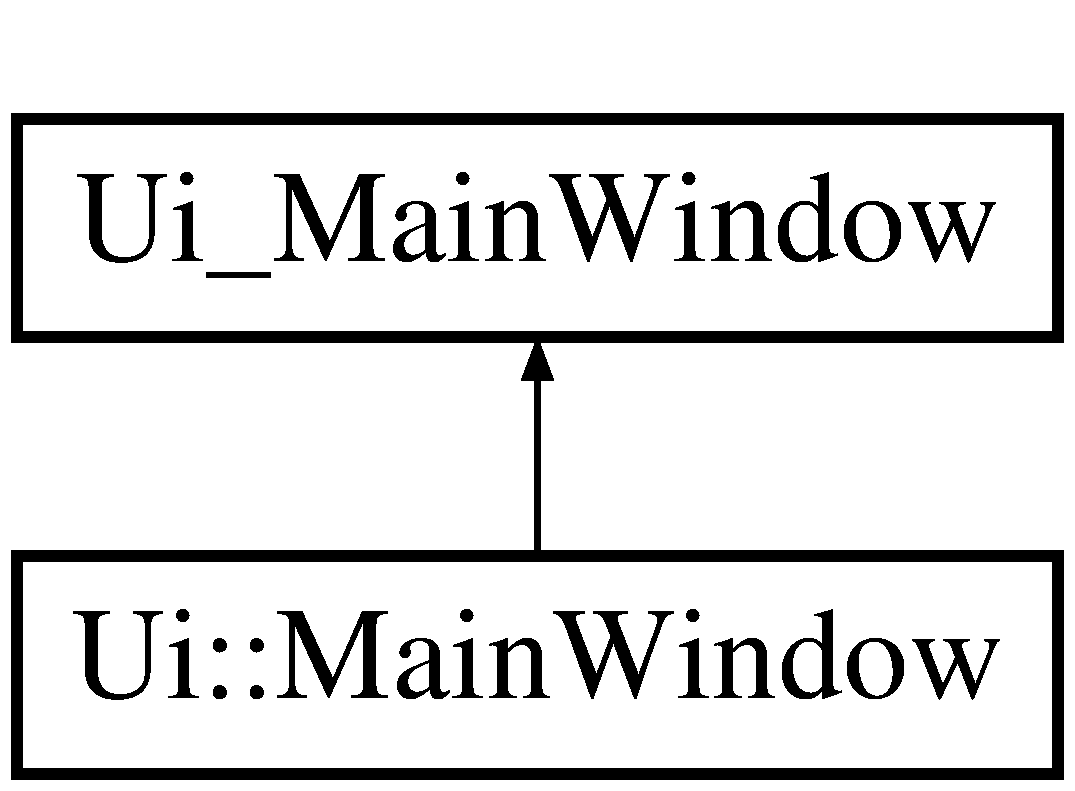
\includegraphics[height=1.454545cm]{class_ui_1_1_main_window}
\end{center}
\end{figure}
\subsection*{Additional Inherited Members}


The documentation for this class was generated from the following file\+:\begin{DoxyCompactItemize}
\item 
C\+:/\+Users/\+Dorgival/\+Desktop/\+Projeto03/build-\/\+Qt\+Server\+Multithread-\/\+Desktop\+\_\+\+Qt\+\_\+5\+\_\+11\+\_\+0\+\_\+\+G\+C\+C\+\_\+64bit-\/\+Debug/ui\+\_\+mainwindow.\+h\end{DoxyCompactItemize}

\section{Main\+Window Class Reference}
\label{class_main_window}\index{Main\+Window@{Main\+Window}}


The \doxyref{Main\+Window}{p.}{class_main_window} class tem a função de comandar as ações de como a interface será trabalhada/operada.  




{\ttfamily \#include $<$mainwindow.\+h$>$}

Inheritance diagram for Main\+Window\+:\begin{figure}[H]
\begin{center}
\leavevmode
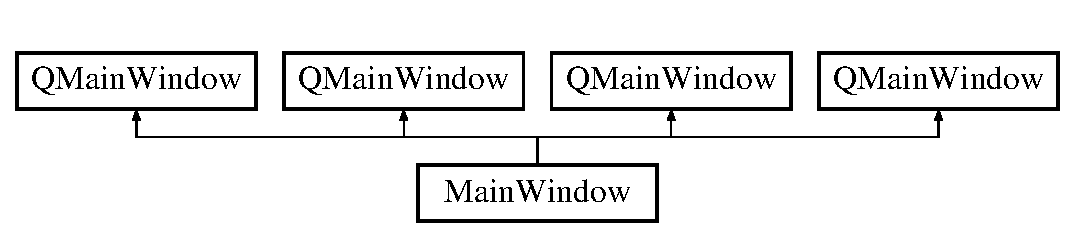
\includegraphics[height=2.000000cm]{class_main_window}
\end{center}
\end{figure}
\subsection*{Public Slots}
\begin{DoxyCompactItemize}
\item 
\mbox{\label{class_main_window_afdfeb13ec363b0eb8ecacaf0aa13b605}} 
void {\bfseries put\+Data} ()
\item 
\mbox{\label{class_main_window_a4a2ddf4cf2ec8e240cc340416b1df792}} 
void {\bfseries get\+Data} ()
\item 
\mbox{\label{class_main_window_ac5b669957c442b6eb68573dacfce33e1}} 
void \textbf{ tcp\+Connect} ()
\begin{DoxyCompactList}\small\item\em tcp\+Connect faz a conexão com o servidor. \end{DoxyCompactList}\item 
\mbox{\label{class_main_window_afdfeb13ec363b0eb8ecacaf0aa13b605}} 
void \textbf{ put\+Data} ()
\begin{DoxyCompactList}\small\item\em put\+Data simula a produção de dados e imprime na tela o dado e o tempo em que ele foi gerado. \end{DoxyCompactList}\item 
\mbox{\label{class_main_window_a4d22c4c7afc7ba0a2fa4c70515c85dda}} 
void \textbf{ tcp\+Disconnect} ()
\begin{DoxyCompactList}\small\item\em tcp\+Disconnect faz o corte da conexão entre o servidor e o produtor. \end{DoxyCompactList}\item 
void \textbf{ mudar\+IP} (Q\+String \+\_\+ip)
\begin{DoxyCompactList}\small\item\em mudar\+IP serve para mudar o ip que, por padrão, é o localhost 127.\+0.\+0.\+1. \end{DoxyCompactList}\item 
void \textbf{ set\+Min} (int \+\_\+min)
\begin{DoxyCompactList}\small\item\em set\+Min configura o valor mínimo na faixa de valores a serem gerados a partir do slider. O set\+Min também impede que o valor máximo seja menor que o mínimo. \end{DoxyCompactList}\item 
void \textbf{ set\+Max} (int \+\_\+max)
\begin{DoxyCompactList}\small\item\em set\+Max configura o valor máximo na faixa de valores a serem gerados a partir do slider. O set\+Max também impede que o valor mínimo seja maior que o máximo. \end{DoxyCompactList}\item 
\mbox{\label{class_main_window_a7fd62e78b41bf758052da7d1451699cb}} 
void \textbf{ init\+Timer} ()
\begin{DoxyCompactList}\small\item\em init\+Timer inicia ou para o contador dos números gerados aleatoriamente. \end{DoxyCompactList}\item 
\mbox{\label{class_main_window_a3ad9aa1924e5560afa1ee473da5c272e}} 
void \textbf{ destroy\+Timer} ()
\begin{DoxyCompactList}\small\item\em destroy\+Timer reseta o timer \end{DoxyCompactList}\item 
void \textbf{ set\+Timer} (int \+\_\+t)
\begin{DoxyCompactList}\small\item\em set\+Timer configura o timer. \end{DoxyCompactList}\item 
\mbox{\label{class_main_window_a0edca0c59fb238bea02b248c90b89698}} 
void {\bfseries show\+Message} (Q\+String msg)
\end{DoxyCompactItemize}
\subsection*{Public Member Functions}
\begin{DoxyCompactItemize}
\item 
\mbox{\label{class_main_window_a8b244be8b7b7db1b08de2a2acb9409db}} 
{\bfseries Main\+Window} (Q\+Widget $\ast$parent=0)
\item 
\mbox{\label{class_main_window_ac5b669957c442b6eb68573dacfce33e1}} 
void {\bfseries tcp\+Connect} ()
\item 
\mbox{\label{class_main_window_a8b244be8b7b7db1b08de2a2acb9409db}} 
{\bfseries Main\+Window} (Q\+Widget $\ast$parent=0)
\item 
\mbox{\label{class_main_window_ac5b669957c442b6eb68573dacfce33e1}} 
void {\bfseries tcp\+Connect} ()
\item 
\textbf{ Main\+Window} (Q\+Widget $\ast$parent=0)
\begin{DoxyCompactList}\small\item\em \doxyref{Main\+Window}{p.}{class_main_window}. \end{DoxyCompactList}\item 
void \textbf{ timer\+Event} (Q\+Timer\+Event $\ast$event)
\begin{DoxyCompactList}\small\item\em timer\+Event faz com que os dados sejam enviados ao servidor \end{DoxyCompactList}\item 
\mbox{\label{class_main_window_a8b244be8b7b7db1b08de2a2acb9409db}} 
{\bfseries Main\+Window} (Q\+Widget $\ast$parent=0)
\end{DoxyCompactItemize}


\subsection{Detailed Description}
The \doxyref{Main\+Window}{p.}{class_main_window} class tem a função de comandar as ações de como a interface será trabalhada/operada. 

\subsection{Constructor \& Destructor Documentation}
\mbox{\label{class_main_window_a8b244be8b7b7db1b08de2a2acb9409db}} 
\index{Main\+Window@{Main\+Window}!Main\+Window@{Main\+Window}}
\index{Main\+Window@{Main\+Window}!Main\+Window@{Main\+Window}}
\subsubsection{Main\+Window()}
{\footnotesize\ttfamily Main\+Window\+::\+Main\+Window (\begin{DoxyParamCaption}\item[{Q\+Widget $\ast$}]{parent = {\ttfamily 0} }\end{DoxyParamCaption})\hspace{0.3cm}{\ttfamily [explicit]}}



\doxyref{Main\+Window}{p.}{class_main_window}. 


\begin{DoxyParams}{Parameters}
{\em parent} & \\
\hline
\end{DoxyParams}


\subsection{Member Function Documentation}
\mbox{\label{class_main_window_aa428a7979ad9beb9c6ebf6478eb611b8}} 
\index{Main\+Window@{Main\+Window}!mudar\+IP@{mudar\+IP}}
\index{mudar\+IP@{mudar\+IP}!Main\+Window@{Main\+Window}}
\subsubsection{mudar\+IP}
{\footnotesize\ttfamily void Main\+Window\+::mudar\+IP (\begin{DoxyParamCaption}\item[{Q\+String}]{\+\_\+ip }\end{DoxyParamCaption})\hspace{0.3cm}{\ttfamily [slot]}}



mudar\+IP serve para mudar o ip que, por padrão, é o localhost 127.\+0.\+0.\+1. 


\begin{DoxyParams}{Parameters}
{\em \+\_\+ip} & é um Qstring que guarda o novo ip a ser colocado. \\
\hline
\end{DoxyParams}
\mbox{\label{class_main_window_ad8a004156f79731b347b744e473006ba}} 
\index{Main\+Window@{Main\+Window}!set\+Max@{set\+Max}}
\index{set\+Max@{set\+Max}!Main\+Window@{Main\+Window}}
\subsubsection{set\+Max}
{\footnotesize\ttfamily void Main\+Window\+::set\+Max (\begin{DoxyParamCaption}\item[{int}]{\+\_\+max }\end{DoxyParamCaption})\hspace{0.3cm}{\ttfamily [slot]}}



set\+Max configura o valor máximo na faixa de valores a serem gerados a partir do slider. O set\+Max também impede que o valor mínimo seja maior que o máximo. 


\begin{DoxyParams}{Parameters}
{\em \+\_\+max} & é o valor recebido pelo slider. \\
\hline
\end{DoxyParams}
\mbox{\label{class_main_window_a32f19952203e037e8022343c290b596f}} 
\index{Main\+Window@{Main\+Window}!set\+Min@{set\+Min}}
\index{set\+Min@{set\+Min}!Main\+Window@{Main\+Window}}
\subsubsection{set\+Min}
{\footnotesize\ttfamily void Main\+Window\+::set\+Min (\begin{DoxyParamCaption}\item[{int}]{\+\_\+min }\end{DoxyParamCaption})\hspace{0.3cm}{\ttfamily [slot]}}



set\+Min configura o valor mínimo na faixa de valores a serem gerados a partir do slider. O set\+Min também impede que o valor máximo seja menor que o mínimo. 


\begin{DoxyParams}{Parameters}
{\em \+\_\+min} & é o valor recebido pelo slider. \\
\hline
\end{DoxyParams}
\mbox{\label{class_main_window_ab5db2dcd9b9592285a18fa7d19256e6a}} 
\index{Main\+Window@{Main\+Window}!set\+Timer@{set\+Timer}}
\index{set\+Timer@{set\+Timer}!Main\+Window@{Main\+Window}}
\subsubsection{set\+Timer}
{\footnotesize\ttfamily void Main\+Window\+::set\+Timer (\begin{DoxyParamCaption}\item[{int}]{\+\_\+t }\end{DoxyParamCaption})\hspace{0.3cm}{\ttfamily [slot]}}



set\+Timer configura o timer. 


\begin{DoxyParams}{Parameters}
{\em \+\_\+t} & valor recebido do slider. \\
\hline
\end{DoxyParams}
\mbox{\label{class_main_window_aaa425b1554af3c1f58cc70b4815082ae}} 
\index{Main\+Window@{Main\+Window}!timer\+Event@{timer\+Event}}
\index{timer\+Event@{timer\+Event}!Main\+Window@{Main\+Window}}
\subsubsection{timer\+Event()}
{\footnotesize\ttfamily void Main\+Window\+::timer\+Event (\begin{DoxyParamCaption}\item[{Q\+Timer\+Event $\ast$}]{event }\end{DoxyParamCaption})}



timer\+Event faz com que os dados sejam enviados ao servidor 


\begin{DoxyParams}{Parameters}
{\em event} & \\
\hline
\end{DoxyParams}


The documentation for this class was generated from the following files\+:\begin{DoxyCompactItemize}
\item 
C\+:/\+Users/\+Dorgival/\+Desktop/\+Projeto03/mainwindow.\+h\item 
C\+:/\+Users/\+Dorgival/\+Desktop/\+Projeto03/mainwindow.\+cpp\end{DoxyCompactItemize}

\hypertarget{class_my_server}{}\section{My\+Server Class Reference}
\label{class_my_server}\index{My\+Server@{My\+Server}}


The \mbox{\hyperlink{class_my_server}{My\+Server}} class inicia um servidor T\+CP capaz de \char`\"{}ouvir\char`\"{} a porta 1234.  




{\ttfamily \#include $<$myserver.\+h$>$}

Inheritance diagram for My\+Server\+:\begin{figure}[H]
\begin{center}
\leavevmode
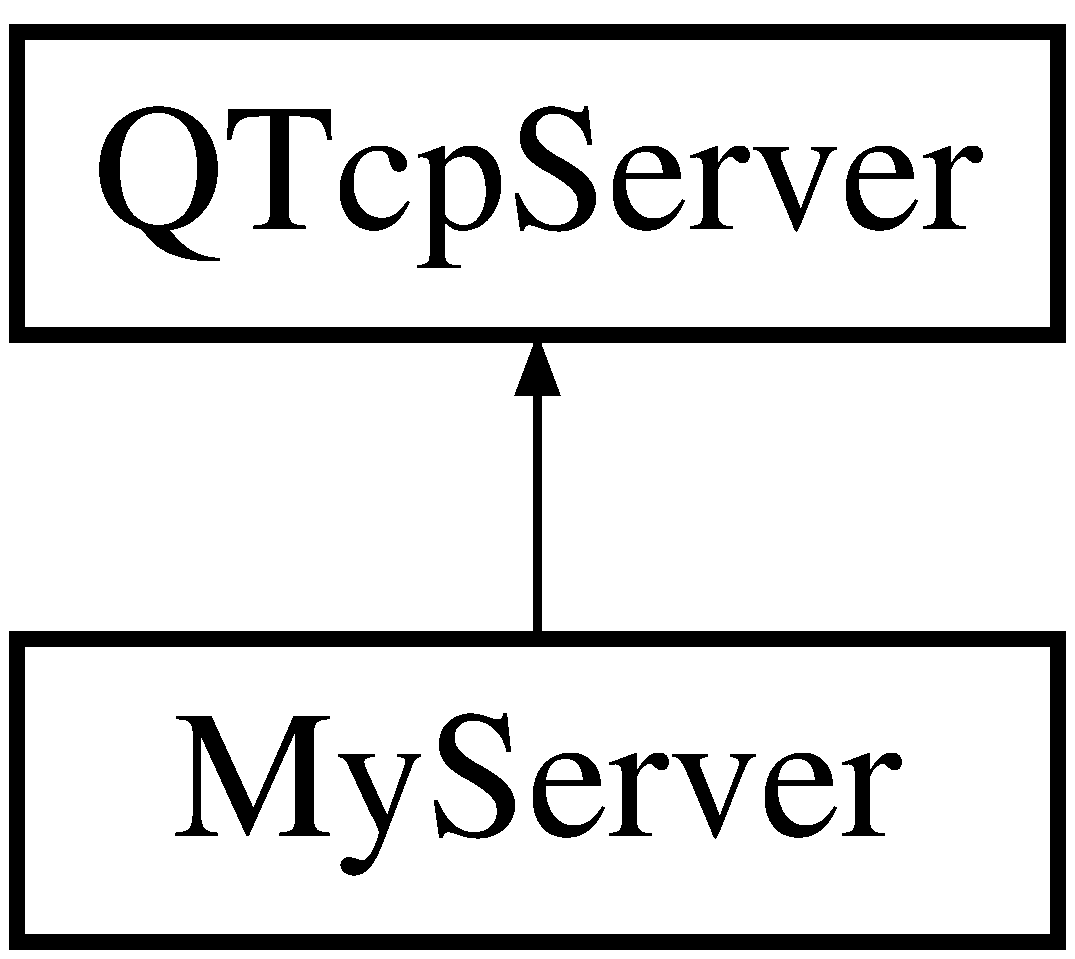
\includegraphics[height=2.000000cm]{class_my_server}
\end{center}
\end{figure}
\subsection*{Public Slots}
\begin{DoxyCompactItemize}
\item 
\mbox{\Hypertarget{class_my_server_ac795ee6f1607c0fa4e635a0da2bf2164}\label{class_my_server_ac795ee6f1607c0fa4e635a0da2bf2164}} 
void {\bfseries receive\+Msg} (Q\+String str)
\end{DoxyCompactItemize}
\subsection*{Signals}
\begin{DoxyCompactItemize}
\item 
\mbox{\Hypertarget{class_my_server_a2b884bce37840b1b461363a37b463b30}\label{class_my_server_a2b884bce37840b1b461363a37b463b30}} 
void {\bfseries message} (Q\+String)
\end{DoxyCompactItemize}
\subsection*{Public Member Functions}
\begin{DoxyCompactItemize}
\item 
\mbox{\hyperlink{class_my_server_ac9e5ca7b551a5df90d5b39260f7e5404}{My\+Server}} (Q\+Object $\ast$parent=0)
\begin{DoxyCompactList}\small\item\em \mbox{\hyperlink{class_my_server}{My\+Server}} é o construtor da classe. \end{DoxyCompactList}\item 
\mbox{\Hypertarget{class_my_server_a962f0e205a0aaf08b12d50d1315a8c90}\label{class_my_server_a962f0e205a0aaf08b12d50d1315a8c90}} 
void \mbox{\hyperlink{class_my_server_a962f0e205a0aaf08b12d50d1315a8c90}{start\+Server}} ()
\begin{DoxyCompactList}\small\item\em Start\+Server start the T\+CP server. \end{DoxyCompactList}\item 
Q\+String\+List \mbox{\hyperlink{class_my_server_ac10d498dcc2b5d691f131f17b6602a59}{get\+I\+P\+List}} ()
\begin{DoxyCompactList}\small\item\em get\+I\+P\+List return a list of I\+Ps used by server \end{DoxyCompactList}\end{DoxyCompactItemize}
\subsection*{Protected Member Functions}
\begin{DoxyCompactItemize}
\item 
void \mbox{\hyperlink{class_my_server_a635c7a1e6817285ffb1a2a3842df010b}{incoming\+Connection}} (qintptr socket\+Descriptor)
\begin{DoxyCompactList}\small\item\em incoming\+Connection decide o que fazer quando uma nova conexao é iniciada \end{DoxyCompactList}\end{DoxyCompactItemize}


\subsection{Detailed Description}
The \mbox{\hyperlink{class_my_server}{My\+Server}} class inicia um servidor T\+CP capaz de \char`\"{}ouvir\char`\"{} a porta 1234. 

\subsection{Constructor \& Destructor Documentation}
\mbox{\Hypertarget{class_my_server_ac9e5ca7b551a5df90d5b39260f7e5404}\label{class_my_server_ac9e5ca7b551a5df90d5b39260f7e5404}} 
\index{My\+Server@{My\+Server}!My\+Server@{My\+Server}}
\index{My\+Server@{My\+Server}!My\+Server@{My\+Server}}
\subsubsection{\texorpdfstring{My\+Server()}{MyServer()}}
{\footnotesize\ttfamily My\+Server\+::\+My\+Server (\begin{DoxyParamCaption}\item[{Q\+Object $\ast$}]{parent = {\ttfamily 0} }\end{DoxyParamCaption})}



\mbox{\hyperlink{class_my_server}{My\+Server}} é o construtor da classe. 


\begin{DoxyParams}{Parameters}
{\em parent} & eh o pai do objeto (nao usado) \\
\hline
\end{DoxyParams}


\subsection{Member Function Documentation}
\mbox{\Hypertarget{class_my_server_ac10d498dcc2b5d691f131f17b6602a59}\label{class_my_server_ac10d498dcc2b5d691f131f17b6602a59}} 
\index{My\+Server@{My\+Server}!get\+I\+P\+List@{get\+I\+P\+List}}
\index{get\+I\+P\+List@{get\+I\+P\+List}!My\+Server@{My\+Server}}
\subsubsection{\texorpdfstring{get\+I\+P\+List()}{getIPList()}}
{\footnotesize\ttfamily Q\+String\+List My\+Server\+::get\+I\+P\+List (\begin{DoxyParamCaption}{ }\end{DoxyParamCaption})}



get\+I\+P\+List return a list of I\+Ps used by server 

\begin{DoxyReturn}{Returns}

\end{DoxyReturn}
\mbox{\Hypertarget{class_my_server_a635c7a1e6817285ffb1a2a3842df010b}\label{class_my_server_a635c7a1e6817285ffb1a2a3842df010b}} 
\index{My\+Server@{My\+Server}!incoming\+Connection@{incoming\+Connection}}
\index{incoming\+Connection@{incoming\+Connection}!My\+Server@{My\+Server}}
\subsubsection{\texorpdfstring{incoming\+Connection()}{incomingConnection()}}
{\footnotesize\ttfamily void My\+Server\+::incoming\+Connection (\begin{DoxyParamCaption}\item[{qintptr}]{socket\+Descriptor }\end{DoxyParamCaption})\hspace{0.3cm}{\ttfamily [protected]}}



incoming\+Connection decide o que fazer quando uma nova conexao é iniciada 


\begin{DoxyParams}{Parameters}
{\em socket\+Descriptor} & é o identificador do socket para a conexao \\
\hline
\end{DoxyParams}


The documentation for this class was generated from the following files\+:\begin{DoxyCompactItemize}
\item 
C\+:/\+Users/dorgi/\+Desktop/\+Projeto03/\+Qt\+Tcp\+Server/myserver.\+h\item 
C\+:/\+Users/dorgi/\+Desktop/\+Projeto03/\+Qt\+Tcp\+Server/moc\+\_\+myserver.\+cpp\item 
C\+:/\+Users/dorgi/\+Desktop/\+Projeto03/\+Qt\+Tcp\+Server/myserver.\+cpp\end{DoxyCompactItemize}

\hypertarget{class_my_thread}{}\section{My\+Thread Class Reference}
\label{class_my_thread}\index{My\+Thread@{My\+Thread}}


The \mbox{\hyperlink{class_my_thread}{My\+Thread}} class cria uma thread que lida com o tratamento de uma conexao T\+CP de entrada.  




{\ttfamily \#include $<$mythread.\+h$>$}

Inheritance diagram for My\+Thread\+:\begin{figure}[H]
\begin{center}
\leavevmode
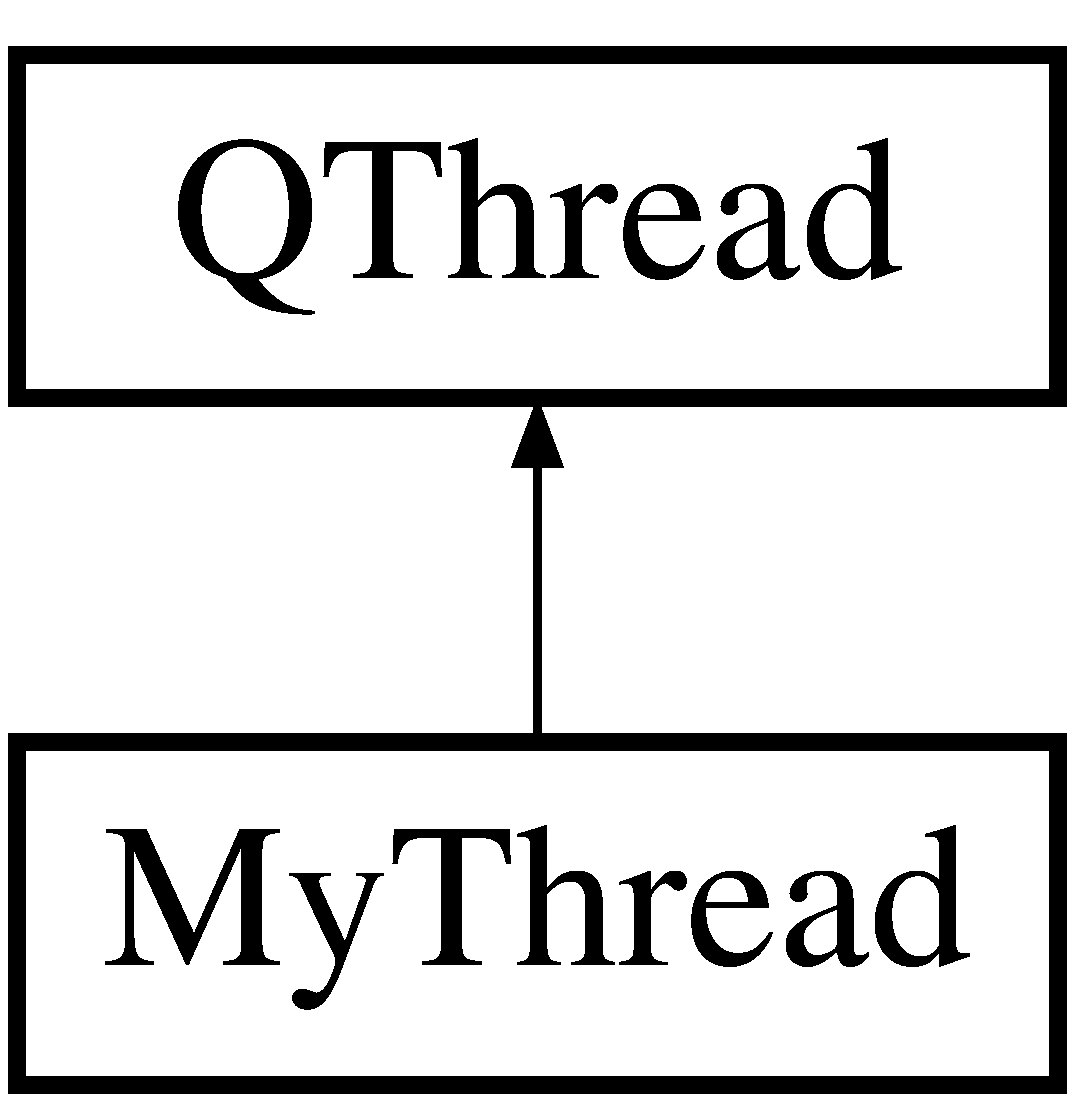
\includegraphics[height=2.000000cm]{class_my_thread}
\end{center}
\end{figure}
\subsection*{Public Slots}
\begin{DoxyCompactItemize}
\item 
\mbox{\Hypertarget{class_my_thread_a277618fdd448b927f2e250c2076fc176}\label{class_my_thread_a277618fdd448b927f2e250c2076fc176}} 
void {\bfseries ready\+Read} ()
\item 
\mbox{\Hypertarget{class_my_thread_a447710039787ae20134a9b572487840f}\label{class_my_thread_a447710039787ae20134a9b572487840f}} 
void {\bfseries disconnected} ()
\end{DoxyCompactItemize}
\subsection*{Signals}
\begin{DoxyCompactItemize}
\item 
\mbox{\Hypertarget{class_my_thread_aebf11d93838f22c9547d0c6aa97002be}\label{class_my_thread_aebf11d93838f22c9547d0c6aa97002be}} 
void {\bfseries error} (Q\+Tcp\+Socket\+::\+Socket\+Error socketerror)
\item 
\mbox{\Hypertarget{class_my_thread_ae49528d4ec1b2208240f707f5aa74adf}\label{class_my_thread_ae49528d4ec1b2208240f707f5aa74adf}} 
void {\bfseries message} (Q\+String)
\end{DoxyCompactItemize}
\subsection*{Public Member Functions}
\begin{DoxyCompactItemize}
\item 
\mbox{\hyperlink{class_my_thread_ac1b04b0fa6b32038e810c7105ef762f6}{My\+Thread}} (int ID, Q\+Object $\ast$parent, \mbox{\hyperlink{class_data_storage}{Data\+Storage}} $\ast$storage)
\begin{DoxyCompactList}\small\item\em \mbox{\hyperlink{class_my_thread}{My\+Thread}} eh o construtor da classe. \end{DoxyCompactList}\item 
\mbox{\Hypertarget{class_my_thread_a48f2e366e852087c53705f64e1ee65c2}\label{class_my_thread_a48f2e366e852087c53705f64e1ee65c2}} 
void {\bfseries run} ()
\end{DoxyCompactItemize}


\subsection{Detailed Description}
The \mbox{\hyperlink{class_my_thread}{My\+Thread}} class cria uma thread que lida com o tratamento de uma conexao T\+CP de entrada. 

\subsection{Constructor \& Destructor Documentation}
\mbox{\Hypertarget{class_my_thread_ac1b04b0fa6b32038e810c7105ef762f6}\label{class_my_thread_ac1b04b0fa6b32038e810c7105ef762f6}} 
\index{My\+Thread@{My\+Thread}!My\+Thread@{My\+Thread}}
\index{My\+Thread@{My\+Thread}!My\+Thread@{My\+Thread}}
\subsubsection{\texorpdfstring{My\+Thread()}{MyThread()}}
{\footnotesize\ttfamily My\+Thread\+::\+My\+Thread (\begin{DoxyParamCaption}\item[{int}]{ID,  }\item[{Q\+Object $\ast$}]{parent,  }\item[{\mbox{\hyperlink{class_data_storage}{Data\+Storage}} $\ast$}]{storage }\end{DoxyParamCaption})}



\mbox{\hyperlink{class_my_thread}{My\+Thread}} eh o construtor da classe. 


\begin{DoxyParams}{Parameters}
{\em ID} & eh o identificador da thread \\
\hline
{\em parent} & \\
\hline
{\em storage} & \\
\hline
\end{DoxyParams}


The documentation for this class was generated from the following files\+:\begin{DoxyCompactItemize}
\item 
C\+:/\+Users/dorgi/\+Desktop/\+Projeto03/\+Qt\+Tcp\+Server/mythread.\+h\item 
C\+:/\+Users/dorgi/\+Desktop/\+Projeto03/\+Qt\+Tcp\+Server/moc\+\_\+mythread.\+cpp\item 
C\+:/\+Users/dorgi/\+Desktop/\+Projeto03/\+Qt\+Tcp\+Server/mythread.\+cpp\end{DoxyCompactItemize}

\hypertarget{structqt__meta__stringdata___main_window__t}{}\section{qt\+\_\+meta\+\_\+stringdata\+\_\+\+Main\+Window\+\_\+t Struct Reference}
\label{structqt__meta__stringdata___main_window__t}\index{qt\+\_\+meta\+\_\+stringdata\+\_\+\+Main\+Window\+\_\+t@{qt\+\_\+meta\+\_\+stringdata\+\_\+\+Main\+Window\+\_\+t}}
\subsection*{Public Attributes}
\begin{DoxyCompactItemize}
\item 
\mbox{\Hypertarget{structqt__meta__stringdata___main_window__t_a332d7fa058028f7613b5ba68abb5a7fe}\label{structqt__meta__stringdata___main_window__t_a332d7fa058028f7613b5ba68abb5a7fe}} 
Q\+Byte\+Array\+Data {\bfseries data} \mbox{[}4\mbox{]}
\item 
\mbox{\Hypertarget{structqt__meta__stringdata___main_window__t_a10e266ffded4c5e956d35d922fa94828}\label{structqt__meta__stringdata___main_window__t_a10e266ffded4c5e956d35d922fa94828}} 
char {\bfseries stringdata0} \mbox{[}28\mbox{]}
\end{DoxyCompactItemize}


The documentation for this struct was generated from the following file\+:\begin{DoxyCompactItemize}
\item 
C\+:/\+Users/dorgi/\+Desktop/\+Projeto03/\+Qt\+Tcp\+Server/moc\+\_\+mainwindow.\+cpp\end{DoxyCompactItemize}

\section{qt\+\_\+meta\+\_\+stringdata\+\_\+\+My\+Server\+\_\+t Struct Reference}
\label{structqt__meta__stringdata___my_server__t}\index{qt\+\_\+meta\+\_\+stringdata\+\_\+\+My\+Server\+\_\+t@{qt\+\_\+meta\+\_\+stringdata\+\_\+\+My\+Server\+\_\+t}}
\subsection*{Public Attributes}
\begin{DoxyCompactItemize}
\item 
\mbox{\label{structqt__meta__stringdata___my_server__t_a6b8c272a34c9891d4f50bddd2586257b}} 
Q\+Byte\+Array\+Data {\bfseries data} [5]
\item 
\mbox{\label{structqt__meta__stringdata___my_server__t_a7acc3222b181da2fe5755caf57bae2be}} 
char {\bfseries stringdata0} [33]
\item 
\mbox{\label{structqt__meta__stringdata___my_server__t_a78f31261b35445e3897ae8256d655007}} 
char {\bfseries stringdata} [34]
\end{DoxyCompactItemize}


The documentation for this struct was generated from the following file\+:\begin{DoxyCompactItemize}
\item 
C\+:/\+Users/\+Dorgival/\+Desktop/\+Projeto03/build-\/\+Qt\+Server\+Multithread-\/\+Desktop\+\_\+\+Qt\+\_\+5\+\_\+11\+\_\+0\+\_\+\+G\+C\+C\+\_\+64bit-\/\+Debug/moc\+\_\+myserver.\+cpp\end{DoxyCompactItemize}

\hypertarget{structqt__meta__stringdata___my_thread__t}{}\section{qt\+\_\+meta\+\_\+stringdata\+\_\+\+My\+Thread\+\_\+t Struct Reference}
\label{structqt__meta__stringdata___my_thread__t}\index{qt\+\_\+meta\+\_\+stringdata\+\_\+\+My\+Thread\+\_\+t@{qt\+\_\+meta\+\_\+stringdata\+\_\+\+My\+Thread\+\_\+t}}
\subsection*{Public Attributes}
\begin{DoxyCompactItemize}
\item 
\mbox{\Hypertarget{structqt__meta__stringdata___my_thread__t_ab5607f1078333a9d42458336e4f735dd}\label{structqt__meta__stringdata___my_thread__t_ab5607f1078333a9d42458336e4f735dd}} 
Q\+Byte\+Array\+Data {\bfseries data} \mbox{[}8\mbox{]}
\item 
\mbox{\Hypertarget{structqt__meta__stringdata___my_thread__t_aa80f739ca8c1b5cfcf28f7f8d8666688}\label{structqt__meta__stringdata___my_thread__t_aa80f739ca8c1b5cfcf28f7f8d8666688}} 
char {\bfseries stringdata0} \mbox{[}83\mbox{]}
\end{DoxyCompactItemize}


The documentation for this struct was generated from the following file\+:\begin{DoxyCompactItemize}
\item 
C\+:/\+Users/dorgi/\+Desktop/\+Projeto03/\+Qt\+Tcp\+Server/moc\+\_\+mythread.\+cpp\end{DoxyCompactItemize}

\hypertarget{struct_range_test}{}\section{Range\+Test Struct Reference}
\label{struct_range_test}\index{Range\+Test@{Range\+Test}}
\subsection*{Public Member Functions}
\begin{DoxyCompactItemize}
\item 
\mbox{\Hypertarget{struct_range_test_a9d96f82c111ffd4d2747416b90306791}\label{struct_range_test_a9d96f82c111ffd4d2747416b90306791}} 
{\bfseries Range\+Test} (qint64 \+\_\+limit)
\item 
\mbox{\Hypertarget{struct_range_test_add496768a566e04219e840ee25e829d7}\label{struct_range_test_add496768a566e04219e840ee25e829d7}} 
bool {\bfseries operator()} (qint64 n)
\end{DoxyCompactItemize}
\subsection*{Public Attributes}
\begin{DoxyCompactItemize}
\item 
\mbox{\Hypertarget{struct_range_test_a638ebd61c0447db219f10cd1473ab364}\label{struct_range_test_a638ebd61c0447db219f10cd1473ab364}} 
qint64 {\bfseries limit}
\end{DoxyCompactItemize}


The documentation for this struct was generated from the following file\+:\begin{DoxyCompactItemize}
\item 
C\+:/\+Users/dorgi/\+Desktop/\+Projeto03/\+Qt\+Tcp\+Server/datastorage.\+cpp\end{DoxyCompactItemize}

\section{Ui\+\_\+\+Main\+Window Class Reference}
\label{class_ui___main_window}\index{Ui\+\_\+\+Main\+Window@{Ui\+\_\+\+Main\+Window}}
Inheritance diagram for Ui\+\_\+\+Main\+Window\+:\begin{figure}[H]
\begin{center}
\leavevmode
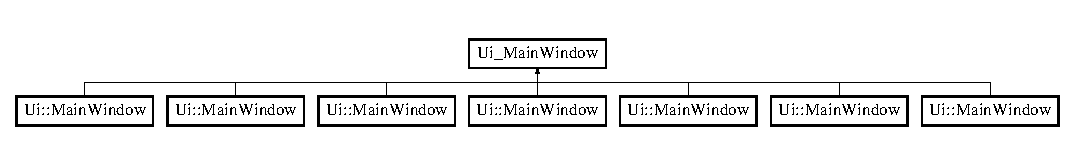
\includegraphics[height=1.454545cm]{class_ui___main_window}
\end{center}
\end{figure}
\subsection*{Public Member Functions}
\begin{DoxyCompactItemize}
\item 
\mbox{\label{class_ui___main_window_acf4a0872c4c77d8f43a2ec66ed849b58}} 
void {\bfseries setup\+Ui} (Q\+Main\+Window $\ast$\textbf{ Main\+Window})
\item 
\mbox{\label{class_ui___main_window_a097dd160c3534a204904cb374412c618}} 
void {\bfseries retranslate\+Ui} (Q\+Main\+Window $\ast$\textbf{ Main\+Window})
\item 
\mbox{\label{class_ui___main_window_acf4a0872c4c77d8f43a2ec66ed849b58}} 
void {\bfseries setup\+Ui} (Q\+Main\+Window $\ast$\textbf{ Main\+Window})
\item 
\mbox{\label{class_ui___main_window_a097dd160c3534a204904cb374412c618}} 
void {\bfseries retranslate\+Ui} (Q\+Main\+Window $\ast$\textbf{ Main\+Window})
\item 
\mbox{\label{class_ui___main_window_acf4a0872c4c77d8f43a2ec66ed849b58}} 
void {\bfseries setup\+Ui} (Q\+Main\+Window $\ast$\textbf{ Main\+Window})
\item 
\mbox{\label{class_ui___main_window_a097dd160c3534a204904cb374412c618}} 
void {\bfseries retranslate\+Ui} (Q\+Main\+Window $\ast$\textbf{ Main\+Window})
\item 
\mbox{\label{class_ui___main_window_acf4a0872c4c77d8f43a2ec66ed849b58}} 
void {\bfseries setup\+Ui} (Q\+Main\+Window $\ast$\textbf{ Main\+Window})
\item 
\mbox{\label{class_ui___main_window_a097dd160c3534a204904cb374412c618}} 
void {\bfseries retranslate\+Ui} (Q\+Main\+Window $\ast$\textbf{ Main\+Window})
\item 
\mbox{\label{class_ui___main_window_acf4a0872c4c77d8f43a2ec66ed849b58}} 
void {\bfseries setup\+Ui} (Q\+Main\+Window $\ast$\textbf{ Main\+Window})
\item 
\mbox{\label{class_ui___main_window_a097dd160c3534a204904cb374412c618}} 
void {\bfseries retranslate\+Ui} (Q\+Main\+Window $\ast$\textbf{ Main\+Window})
\item 
\mbox{\label{class_ui___main_window_acf4a0872c4c77d8f43a2ec66ed849b58}} 
void {\bfseries setup\+Ui} (Q\+Main\+Window $\ast$\textbf{ Main\+Window})
\item 
\mbox{\label{class_ui___main_window_a097dd160c3534a204904cb374412c618}} 
void {\bfseries retranslate\+Ui} (Q\+Main\+Window $\ast$\textbf{ Main\+Window})
\item 
\mbox{\label{class_ui___main_window_acf4a0872c4c77d8f43a2ec66ed849b58}} 
void {\bfseries setup\+Ui} (Q\+Main\+Window $\ast$\textbf{ Main\+Window})
\item 
\mbox{\label{class_ui___main_window_a097dd160c3534a204904cb374412c618}} 
void {\bfseries retranslate\+Ui} (Q\+Main\+Window $\ast$\textbf{ Main\+Window})
\end{DoxyCompactItemize}
\subsection*{Public Attributes}
\begin{DoxyCompactItemize}
\item 
\mbox{\label{class_ui___main_window_a6600dd3bdd3d55e535659e4a4096ea48}} 
Q\+Widget $\ast$ {\bfseries central\+Widget}
\item 
\mbox{\label{class_ui___main_window_ae4fc4a01984f4958d08903a46ce7509a}} 
Q\+H\+Box\+Layout $\ast$ {\bfseries horizontal\+Layout\+\_\+3}
\item 
\mbox{\label{class_ui___main_window_ad396eaa8d855b13559c50e02164b8325}} 
Q\+Group\+Box $\ast$ {\bfseries group\+Box}
\item 
\mbox{\label{class_ui___main_window_ae7104d878681f568e492c5bd0f653157}} 
Q\+H\+Box\+Layout $\ast$ {\bfseries horizontal\+Layout}
\item 
\mbox{\label{class_ui___main_window_a89e0ee00764ef40b900ae0f190644540}} 
Q\+List\+Widget $\ast$ {\bfseries list\+Widget}
\item 
\mbox{\label{class_ui___main_window_a67c4e71bde8605c39057b72d14cbea4b}} 
Q\+Group\+Box $\ast$ {\bfseries group\+Box\+\_\+2}
\item 
\mbox{\label{class_ui___main_window_a9ee21d2c2bc000e7a8ba931bacfc5a69}} 
Q\+H\+Box\+Layout $\ast$ {\bfseries horizontal\+Layout\+\_\+2}
\item 
\mbox{\label{class_ui___main_window_a84c6f864ef5087858db20cf3901746d5}} 
Q\+Text\+Browser $\ast$ {\bfseries text\+Browser}
\item 
\mbox{\label{class_ui___main_window_a502a50d7dc22415f511336bdfb4318b9}} 
Q\+Menu\+Bar $\ast$ {\bfseries menu\+Bar}
\item 
\mbox{\label{class_ui___main_window_abca26371605d7c5235fab5188d4bdcf7}} 
Q\+Tool\+Bar $\ast$ {\bfseries main\+Tool\+Bar}
\item 
\mbox{\label{class_ui___main_window_afa919f3af6f2f526a70f1fa331f63724}} 
Q\+Status\+Bar $\ast$ {\bfseries status\+Bar}
\item 
\mbox{\label{class_ui___main_window_a78edcdd12ea78c06d7e80f322c8882f9}} 
Q\+Label $\ast$ {\bfseries label}
\item 
\mbox{\label{class_ui___main_window_a48fa9370856496c1b53acd023fa8d7b5}} 
Q\+Push\+Button $\ast$ {\bfseries push\+Button\+Connect}
\item 
\mbox{\label{class_ui___main_window_aad9e9965b1b2d32d3eed2743e60cd97e}} 
Q\+Slider $\ast$ {\bfseries horizontal\+Slider\+Timings}
\item 
\mbox{\label{class_ui___main_window_a1ef1c2be2f55c6d3261330e90adfe738}} 
Q\+Slider $\ast$ {\bfseries horizontal\+Slider\+Min}
\item 
\mbox{\label{class_ui___main_window_a7be02f76d2246891df190fe99399f3a7}} 
Q\+Push\+Button $\ast$ {\bfseries push\+Button\+Start}
\item 
\mbox{\label{class_ui___main_window_a3ac482a90bd0760ae9899843eba05ba0}} 
Q\+Push\+Button $\ast$ {\bfseries push\+Button\+Stop}
\item 
\mbox{\label{class_ui___main_window_a2f5576686ce98bcc41bd1b1eca07e56a}} 
Q\+Label $\ast$ {\bfseries label\+\_\+2}
\item 
\mbox{\label{class_ui___main_window_a2b9f1785f6719c063ab248e7428bd074}} 
Q\+Line\+Edit $\ast$ {\bfseries set\+IP}
\item 
\mbox{\label{class_ui___main_window_acb0aaedbb69847beed374d571e9399bf}} 
Q\+L\+C\+D\+Number $\ast$ {\bfseries lcd\+Number\+Min}
\item 
\mbox{\label{class_ui___main_window_a253fbc5b44941384321b7c58cf96cc65}} 
Q\+Label $\ast$ {\bfseries label\+\_\+3}
\item 
\mbox{\label{class_ui___main_window_a953dcd0e658a0903339e2ef3c94d4e7e}} 
Q\+Label $\ast$ {\bfseries label\+\_\+4}
\item 
\mbox{\label{class_ui___main_window_a17fd1ba56a21573669f119f9810a633c}} 
Q\+Slider $\ast$ {\bfseries horizontal\+Slider\+Max}
\item 
\mbox{\label{class_ui___main_window_aaf820c9043e5f5fbaa62322b3a9b2814}} 
Q\+L\+C\+D\+Number $\ast$ {\bfseries lcd\+Number\+Max}
\item 
\mbox{\label{class_ui___main_window_aadc6379583df8659dbbd587a6cae904d}} 
Q\+Push\+Button $\ast$ {\bfseries push\+Button\+Disconnect}
\item 
\mbox{\label{class_ui___main_window_a805d415fff07a22a85219e1f22f2da28}} 
Q\+Widget $\ast$ {\bfseries vertical\+Layout\+Widget}
\item 
\mbox{\label{class_ui___main_window_aecd96a04789fcfec3f98d80390ad8184}} 
Q\+V\+Box\+Layout $\ast$ {\bfseries vertical\+Layout}
\item 
\mbox{\label{class_ui___main_window_aaf97aba343edd00a0114b406c2b77365}} 
Q\+List\+View $\ast$ {\bfseries list\+View}
\item 
\mbox{\label{class_ui___main_window_ab676f235c393f334b7c07935d4007925}} 
Q\+Widget $\ast$ {\bfseries widget}
\item 
\mbox{\label{class_ui___main_window_a0c01bad60d9f422a1258e710635a2f65}} 
Q\+V\+Box\+Layout $\ast$ {\bfseries vertical\+Layout\+\_\+2}
\item 
\mbox{\label{class_ui___main_window_a61dbf7c412581281482647c8814fe82a}} 
Q\+Key\+Sequence\+Edit $\ast$ {\bfseries key\+Sequence\+Edit}
\item 
\mbox{\label{class_ui___main_window_ad28aa003edd69668ad54491ec5a63ccd}} 
Q\+Widget $\ast$ {\bfseries widget1}
\item 
\mbox{\label{class_ui___main_window_a38b8a4b887f3b58e2a49e7905ae6f1f0}} 
Q\+V\+Box\+Layout $\ast$ {\bfseries vertical\+Layout\+\_\+3}
\item 
\mbox{\label{class_ui___main_window_ae183387a7d233b437a637b403ba39ffd}} 
Q\+H\+Box\+Layout $\ast$ {\bfseries horizontal\+Layout\+\_\+4}
\end{DoxyCompactItemize}


The documentation for this class was generated from the following file\+:\begin{DoxyCompactItemize}
\item 
C\+:/\+Users/\+Dorgival/\+Desktop/\+Projeto03/build-\/\+Qt\+Server\+Multithread-\/\+Desktop\+\_\+\+Qt\+\_\+5\+\_\+11\+\_\+0\+\_\+\+G\+C\+C\+\_\+64bit-\/\+Debug/ui\+\_\+mainwindow.\+h\end{DoxyCompactItemize}

%--- End generated contents ---

% Index
\backmatter
\newpage
\phantomsection
\clearemptydoublepage
\addcontentsline{toc}{chapter}{Index}
\printindex

\end{document}
